%!TEX ROOT = main.tex

% Define the process flow charts style
\tikzstyle{block} = [rectangle, draw, fill=blue!20, 
text width=15em, text centered, rounded corners, minimum height=4em]


\chapter{Research Methodology}
\section{Introduction}
This section would illustrate the process flow to carry out the experiments and fulfill the aforementioned objectives of this study. The following flow charts would illustrate the steps taken to conduct the several experiments.

\section{Text preprocessing process flow}
\begin{figure} [ht]
\centering
\begin{tikzpicture}[node distance = 2cm, auto]
% Place nodes
\node [block] (init) {Raw text};
\node [block, below of=init] (readDf) {Read the file into dataframe};
\node [block, below of=readDf] (lineRemoval) {Remove some redundant lines};
\node [block, below of=lineRemoval] (lower) {Convert the text to lowercase};
\node [block, below of=lower] (stopwordRemoval) {Stop words removal};
\node [block, below of=stopwordRemoval] (symRemoval) {Punctuation removal};
\node [block, below of=symRemoval] (lemmatization) {Lemmatization};
\node [block, below of=lemmatization] (output) {Output to CSV file};

% Draw edges

\path [line] (init) -- (readDf);
\path [line] (readDf) -- (lineRemoval);
\path [line] (lineRemoval) -- (lower);
\path [line] (lower) -- (stopwordRemoval);
\path [line] (stopwordRemoval) -- (symRemoval);
\path [line] (symRemoval) -- (lemmatization);
\path [line] (lemmatization) -- (output);
\end{tikzpicture}
\caption{Process flow of preprocessing the news article dataset}
\label{fig: preprocessFlow}
\end{figure}

The flow chart above illustrates the preprocessing process. The news articles dataset is in the form of raw text. Some preprocessing is needed before the features can be extracted from the text to build the text classification models. First, the raw text would be read into a dataframe or a data structure for ease of access and processing.

There are some lines in the raw text files that are irrelevant to text classification, these lines would be removed to reduce the noise in the dataset. All the text in the dataset would be converted to lowercase for uniformity and ease of processing. There are some words in the text that are useful in human speech but do not convey meanings in text analysis. These words are stop words, these words would be removed. After stop words removal, the text should contain only the words that are vital to text analysis but there would be some punctuations and symbols in the text. These punctuations and symbols would be removed as well so that the text is cleaner and less noisy.

After that, there is an important step, lemmatization. Lemmatization would transform most of the words in the text to their root form which is known as a lemma. This would reduce the noise in the data by transforming similar words into a single word. The alternative to lemmatization would be stemming. Stemming would be faster and need less processing power than lemmatization but stemming has a drawback. The result of stemming may not be a real word because stemming just chop off the end of the words thus the resulting words may not be a real words. On the other hand, lemmatization uses vocabulary and morphological analysis of words to remove the inflectional endings only and resulting the root form of words. \cite{stemLemma} Therefore, the output of lemmatization would be better than stemming.

The purpose of lemmatization is to reduced the number of distinct words in the document. The words, "good", "better", and "best" might appear in a news articles dataset. Without lemmatization, these words would be 3 distinct words. With lemmatization, all 3 of these words would be transformed to their root word which is "good". Therefore, by using lemmatization, the number of distinct words in the text would be reduced and the noise in the data would be minimized.

After all the words in the text file are lemmatized, the dataframe that contains the text is written to a CSV file. The training process would be able to read the CSV file easily and train the classification models with the method chosen.\\


\section{Overall Process Flow}
\begin{figure} [ht]
\centering
\begin{tikzpicture} [node distance = 2cm, auto]
% Place nodes
\node [block] (init) {News articles};
\node [block, below of=init] (preprocessing) {Preprocessing};
\node [block, below of=preprocessing] (feaext) {Feature extraction};
\node [block, below of=feaext] (dimred) {Dimension reduction (if needed)};
\node [block, below of=dimred] (ml) {Train machine learning models};
\node [block, below of=ml] (test) {Test the models};
\node [block, below of=test] (eval) {Evaluate the performance};
% Draw edges
\path [line] (init) -- (preprocessing);
\path [line] (preprocessing) -- (feaext);
\path [line] (feaext) -- (dimred);
\path [line] (dimred) -- (ml);
\path [line] (ml) -- (test);
\path [line] (test) -- (eval);

\end{tikzpicture}
\caption{Overall process flow}
\label{fig: overallFlow}
\end{figure}

The process flow chart above is the overall process for the few experiments. As mentioned above, the news articles dataset has to be preprocessed before it can undergo feature extraction and being used to train machine learning models.

After preprocessing, the resulting data would be used in several experiments with a few subtle differences.
The differences in the experiments would be in the feature extraction stage and the dimension reduction stage. 

There would be 2 different document representation method or feature extraction method in the experiments. An experiment would be conducted with each of the feature extraction method without dimension reduction. Several classification models would be trained with the features from both of the feature extraction methods without dimension reduction. By evaluating the performance of the classification models, a more optimized feature extraction method would be identified.

In a number of experiments, the feature matrix output of the 2 feature extraction method would undergo dimension reduction. There is a parameter to the dimension reduction methods to control to what extends should the feature matrix be reduced to. By manipulating this parameter, feature matrices of different dimension would be produced. These matrices with different dimension would be used as training data for classification models. Different dimension of the feature matrices would certainly has an effect on the performance of the classification models. The performance of the classification models trained with feature matrices of different dimension would be evaluated. Thus, the effect of dimension reduction has on the performance of classification models could be determined.

Since there are 2 document representation method and 2 dimension reduction method, there would be a combination of 4 experiments. In addition to the experiments without dimension reduction, there would be a total of 6 experiments. These experiments use different combination of document representation method, dimension reductions and all the 3 classification models. From the results of all the experiments, the best combination of document representation, dimension reduction and classification models for news articles would be identified.

\section{The dataset}
\graphicspath{{./images/}}

The dataset used in this research is the 20 news group dataset. It is freely available at \url{http://qwone.com/~jason/20Newsgroups/}. It is a collection of news articles that can be divided almost evenly to 20 groups. Some of the groups are closely related to one another and some are widely different. Categories with the same prefix for example \textit{comp} would have high similarity with one another but also subtle differences. The categories with the different prefixes, for example \textit{rec} and \textit{talk} would be very different from one another.

This characteristic of the dataset make it a good dataset to test text classification. A good classification model should be able to differentiate the different groups of news article even the groups that closely resembled one another.

The table below show the number of count for each category. There is a total of 18790 articles and most of the categories have almost 1000 articles in them. 

\begin{table} [ht]
	\centering
	\begin{tabular} {|| c | c ||}
		\hline
		Category & count \\ [0.5ex]
		\hline\hline
		alt.atheism & 798 \\
		comp.graphics & 970 \\
		comp.os.ms-windows.misc & 980 \\
		comp.sys.ibm.pc.hardware & 978 \\
		comp.sys.mac.hardware & 957 \\
		comp.windows.x & 978 \\
		misc.forsale & 962 \\
		rec.autos & 988 \\
		rec.motorcycles & 993 \\
		rec.sport.baseball & 993 \\
		rec.sport.hockey & 998 \\
		sci.crypt & 991 \\
		sci.electronics & 981 \\
		sci.med & 988 \\
		sci.space & 986 \\
		soc.religion.christian & 997 \\
		talk.politics.guns & 910 \\
		talk.politics.mideast & 940 \\
		talk.politics.misc & 774 \\
		talk.religion.misc & 628 \\
		\hline
	\end{tabular}
	\caption{The count of each category in the dataset}
	\label{tbl:freqCount}
\end{table}


The bar chart below visualized the data displayed on the table for ease of viewing. Most of categories have almost 1000 articles except alt.atheism, talk.politics.misc and talk.religion.misc.

\begin{figure} [ht]
	\centering
	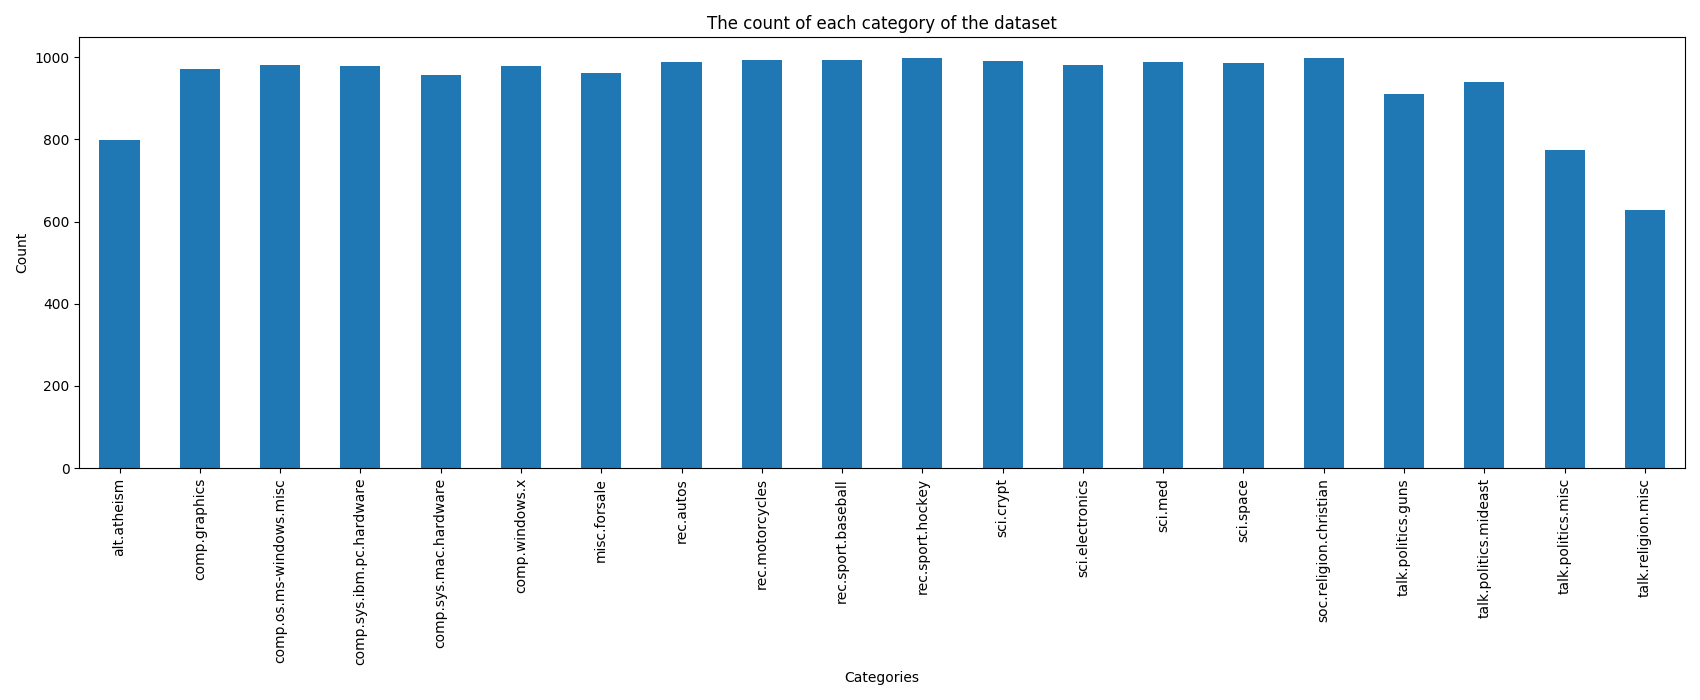
\includegraphics[width=\textwidth]{count}
	\caption{The count of each category in the dataset}
	\label{fig:freqCount}
\end{figure}

As mentioned there are 18790 articles in the data, the articles would be split at random into 8:2 ratio. 80\% of the data would be used as training data to train the classification model while 20\% of the data would be use as the test data. The training data would consist of 15032 articles while the test data would consist of 3758 articles.\\


\section{The experiments}
The experiments that has been conducted in this research is as follows:
\begin{enumerate}
	\item Term frequency
	\item Term frequency with naive dimension reduction
	\item Term frequency with truncated SVD
	\item TF-IDF
	\item TF-IDF with naive dimension reduction
	\item TF-IDF with truncated SVD
\end{enumerate}

Basically, there are 2 feature extraction method used in the experiments, namely term frequency and term frequency - inverse document frequency (\ac{tfidf}). Each of the feature extraction method would be tested with and without dimension reduction algorithm.

There are 2 dimension reduction algorithms involved, one is a naive method, which means that the features or columns lesser than a certain value would be removed. In other words, words or terms that do not appear much in the dataset would be removed. Another dimension reduction algorithm is truncated single value decomposition (\ac{svd}). This method would retain the essence of the data, the part of the data with maximum variance. 

After feature extraction and dimension reduction (if needed) are applied, the resulting features would be used to train text classification models. There are 3 text classification algorithms chosen in these experiments namely k-nearest neighbour (\ac{knn}), support vector machine (\ac{svm}), and neural network (\ac{nn}). All 3 of the machine algorithms would be applied to all the different resulting features and the accuracy scores would be evaluated.


\section{Conclusion}
With the method mentioned above, the experiments would be carry out and the results would be recorded. The results would be compared and the differences would be analysed.